\chapter{Evaluation}
\label{ch:evaluation}

\begin{draft}
GLMTK by me was used for evaluation.

Experiment with runtime of $\ProbGLM{w_n}{w_1^{n-1}}$ from $n=1$ to some upper
bound to showcase complexity improvement of weighted sum to na{\"\i}ve,
recursive approach.

Experiment with top-k join algorithm vs stupid weighted sum argmax, to showcase
runtime improvement of top-k join.

Experiment to showcase (dis-)advantages of GLM to MKN.

Maybe Speedup-factor over time.

Experiments that combine metrices.

Experiments over time and space complexity.
\end{draft}

% ------------------------------------------------------------------------------
\section{Experimental setup}

% ------------------------------------------------------------------------------
\section{Estimator time}

\begin{figure}
  \centering
  \documentclass{standalone}
\usepackage[dvipsnames,svgnames,x11names]{xcolor}
\usepackage{tikz}
\usepackage{pgfplots}
\pgfplotsset{compat = 1.12}
\usepackage{../thesismath}
\begin{document}
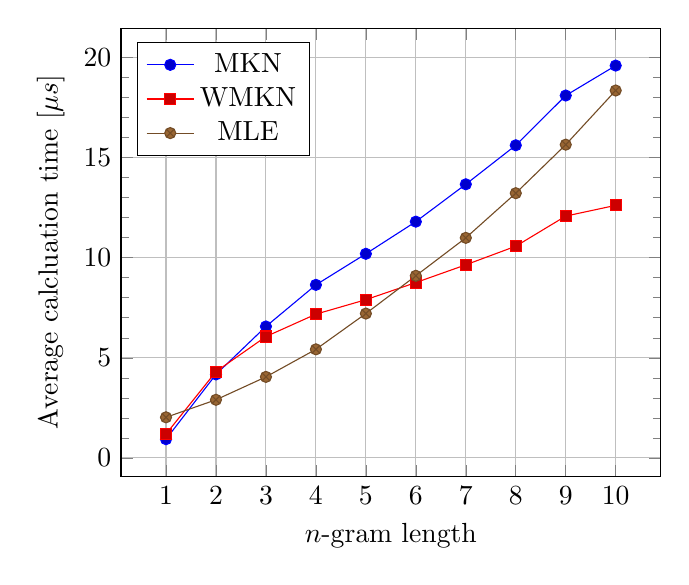
\begin{tikzpicture}[baseline]

\begin{axis}[
  xlabel = {$n$-gram length},
  xtick = {1, ..., 10},
  ylabel = {Average calcluation time [${\mu}s$]},
  minor y tick num = 4,
  grid = major,
  legend entries = {{MKN}, {WMKN}, {MLE}},
  legend pos = north west,
]

% MKN
\addplot table {
  n   us
  % sampled at N = 1000
  1    0.936
  2    4.171
  3    6.565
  4    8.643
  5   10.194
  6   11.800
  7   13.666
  8   15.614
  9   18.099
  10  19.594
};

% WMKN
\addplot table {
  n   us
  % sampled at N = 1000
  1    1.192
  2    4.311
  3    6.060
  4    7.180
  5    7.902
  6    8.758
  7    9.644
  8   10.573
  9   12.078
  10  12.614
};

% MKN
\addplot table {
  n   us
  % sampled at N = 1000
  1    2.028
  2    2.903
  3    4.047
  4    5.423
  5    7.210
  6    9.096
  7   10.991
  8   13.221
  9   15.645
  10  18.350
};

\end{axis}

\end{tikzpicture}
\end{document}

  \caption{\todo[inline]{TimeMKN-Caption}}
\end{figure}

\begin{figure}
  \centering
  \documentclass{standalone}
\usepackage[dvipsnames,svgnames,x11names]{xcolor}
\usepackage{tikz}
\usepackage{pgfplots}
\pgfplotsset{compat = 1.12}
\usepackage{../thesismath}
\begin{document}
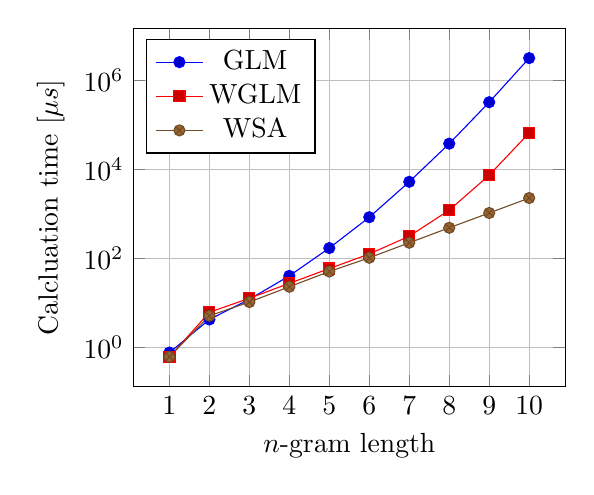
\begin{tikzpicture}[baseline]

\begin{axis}[
  xlabel = {$n$-gram length},
  xtick = {1, ..., 10},
  ylabel = {Calcluation time [${\mu}s$]},
  ymode = log,
  %yticklabel pos = right,
  minor y tick num = 4,
  grid = major,
  legend entries = {{GLM}, {WGLM}, {WSA}},
  legend pos = north west,
  scale = 0.8,
]

% GLM
\addplot table {
  n   us
  % sampled at N = 1000
  1   0.776
  2   4.296
  3   12.188
  4   40.981
  5   172.271
  % sampled at N = 100
  6   848.550
  7   5297.308
  % sampled at N = 10
  8   38045.228
  9   323947.490
  % sampled at N = 1
  10  3168612.887
};

% WGLM
\addplot table {
  n   us
  % sampled at N = 1000
  1   0.618
  2   6.223
  3   12.855
  4   27.786
  5   59.746
  % sampled at N = 100
  6   126.934
  7   317.936
  8   1223.680
  9   7463.531
  10  66226.605
};

% WSA
\addplot table {
  n   us
  % sampled at N = 1000
  1   0.624
  2   5.200
  3   10.572
  4   23.295
  5   51.307
  % sampled at N = 100
  6   104.217
  7   226.905
  8   491.327
  9   1056.845
  10  2287.351
};

\end{axis}

\end{tikzpicture}
\end{document}

  \caption{\todo[inline]{TimeGLM-Caption}}
\end{figure}
